\documentclass{article}
\usepackage{graphicx}
\begin{document}
\noindent
\section{Introduction}

Solid state pixel array detectors have thick sensors relative to their
pixel size in order to obtain good quantum efficiency of
detection. This gives rise to a shift in the position where a photon
is \emph{recorded} with respect to it's intersection with the detector
face, which becomes more pronounced as the angle between the incoming
ray and the detector normal increaases. This parallax correction is
modest (under a pixel) for conventional energies used in MX with
standard sensor thickness, but can become much more pronounced at high
energy.

XDS produces correction tables \verb|X-CORRECTIONS.cbf| and
\verb|Y-CORRECTIONS.cbf| to account for this, which give a shift
between the ideal pixel position and the effective mm position
allowing for this parallax correction. For DIALS such a correction is
necessary in order to most accurately model the detector behaviour.

\section{Acknowledgment}

The initial calculations(i.e. earlier versions of this document) were
frustrated by trying to reproduce the correction tables from XDS -
this will be revisited below. Having got in touch with DECTRIS, Peter
Trueb provided an equation for the parallax correction which is also
rederived below which however disagrees with XDS. It was felt the only
way to address this disagreement was to reverse engineer the XDS model
to allow a direct comparison\footnote{It is worth noting here that
  the XDS model was felt a good basis, as it is currently in
  widespread use for processing X-ray diffraction data from pixel
  array detectors.}.

\section{Terminology}

In an effort to be clear the terminology must be consistent, so the
following definitions are used:

\begin{itemize}
\item{$t_0$ sensor thickness}
\item{$\theta$ angle between incoming ray and detector normal}
\item{$\mu$ attenuation coefficient, i.e. probability of $e^{-\mu x}$ of photon reaching depth $x$ in material}
\item{$t$ apparent thickness equal to $\frac{t_0}{\cos \theta}$}
\end{itemize}

\noindent
In all cases lengths are in mm, so $\mu$ is scaled to $\rm{mm}^{-1}$.

\section{XDS Model}

The XDS model (below) was calculated using the XDS XYCORR step,
however unlike the conventional use case the array was calculated at
full image resolution by multiplying by four the number of pixels in
both directions and dividing by four the pixel size - this then gave
integer CBF images in units of $\frac{1}{40}$ pixel. Once rescaled these
were used for direct comparison.

{
\centering
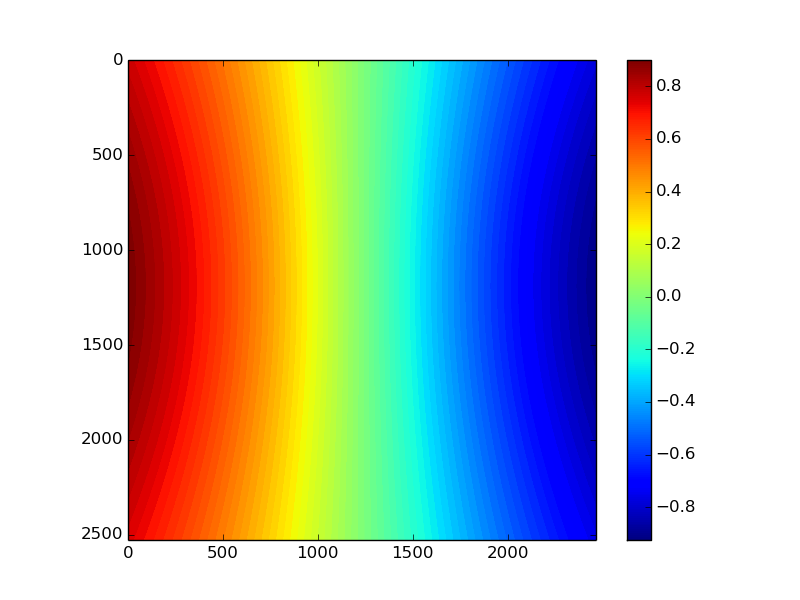
\includegraphics[scale=0.3]{xds_parallax_x.png}
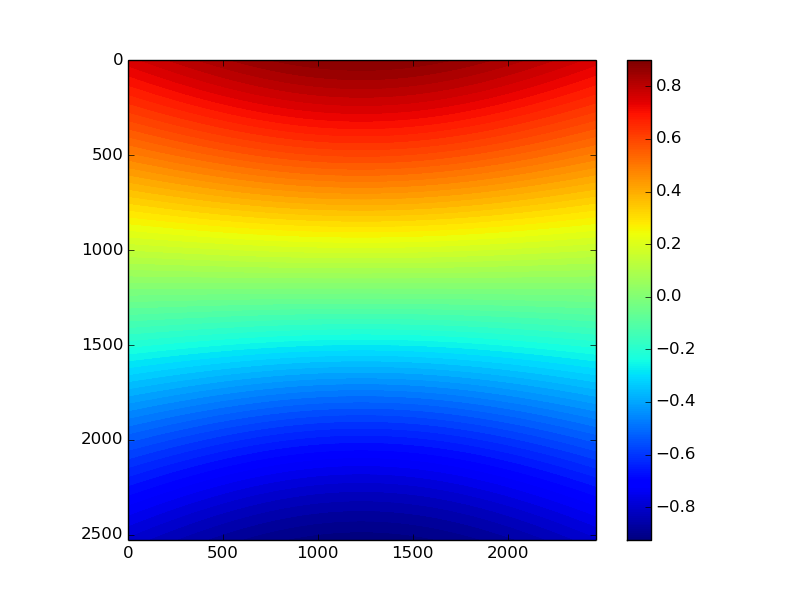
\includegraphics[scale=0.3]{xds_parallax_y.png}
}

\noindent
For reference these were derived from the following \verb|XDS.INP|:

{\small
\begin{verbatim}
JOB=XYCORR
DETECTOR=PILATUS MINIMUM_VALID_PIXEL_VALUE=0 OVERLOAD=161977
DIRECTION_OF_DETECTOR_X-AXIS=1.000 0.000 0.000
DIRECTION_OF_DETECTOR_Y-AXIS=0.000 -1.000 0.000
TRUSTED_REGION=0.0 1.41
NX=9852 NY=10108 QX=0.0430 QY=0.0430
DETECTOR_DISTANCE=265.27
X-RAY_WAVELENGTH=0.976250
INCIDENT_BEAM_DIRECTION=-0.000 -0.000 -1.000
SILICON= 3.984
SENSOR_THICKNESS= 0.320
ORGX=4901.40 ORGY=4773.88
\end{verbatim}
}

\noindent
and correspond to measured data. The \verb|SILICON=| was assigned
from NIST values as this was found to be slightly different when
derived from XDS itself (3.670 in this instance). 

\section{Analytical Model}

The initial analytical model worked out was incorrect, in that the
initial approach was incorrect. As mentioned above, Peter Trueb
provided a better derivation as follows:

\begin{equation}
\frac{I(x)}{I_0} = e^{- \mu x}
\end{equation}

\noindent
so probability of photon being absorbed between $x$ and $x + \delta x$
is

\begin{equation}
p(x) dx = - frac{d \frac{I(x)}{I_0}}{dx} = \mu e^{- \mu x} dx
\end{equation}

\noindent
therefore 

\begin{equation}
<x> = \int_0^t x p(x) dx = \left[ - \left( \frac{1}{\mu} + x \right) 
e^{- \mu x} \right]_0^t
\end{equation}

\noindent
i.e.

\begin{equation}
<x> = \frac{1}{\mu} - \left( t + \frac{1}{\mu} \right) e^{- \mu t}
\end{equation}

\noindent
for the offset this is simply equal to $\sin \theta <x>$, and $t =
\frac{t_0}{\cos \theta}$ so

\begin{equation}
<o> = \sin \theta \left( \frac{1}{\mu} - \left( \frac{t_0}{\cos
      \theta} + \frac{1}{\mu} \right) e^{- \frac{\mu t_0}{\cos \theta}} \right)
\end{equation}


\section{XDS Model Analysis}

Analysis of this model as a function of different scattering angles,
energies and sensor thickness values indicated that the model for the
absolute offset $<o>$ is

\begin{equation}
<o> = \rm{min}\left(\frac{\sin \theta}{\mu}, t_0 \tan \theta \right)
\end{equation}

\noindent
This seems rather ad-hoc to me but does agree well when there is a
high DQE i.e. the sensor is thick or the energy is low.

\section{Example Results}

Following examples are calculated from an example data set recorded on
Diamond I04 with a $320 \rm{\mu m}$ thickness sensor, but with the
energy set from 4keV to 18keV in 1keV steps. Here follow plots for 8,
10, 12, 14, 16 and 18keV. The XDS numerical results (i.e. derived from
the correction tables) are shown in dark blue, the model above in pale
blue and the assumed analytical form of the XDS model in red - clearly
the last of these runs through the centre of the first, and the second
deviates substantially at higher energy.

{
\centering
\begin{tabular}{cc}
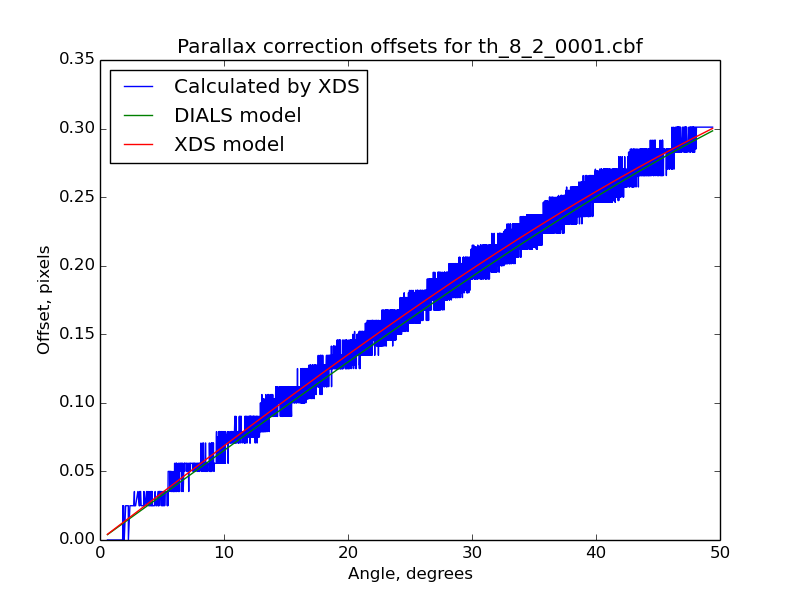
\includegraphics[scale=0.3]{corrections8000.png} & 
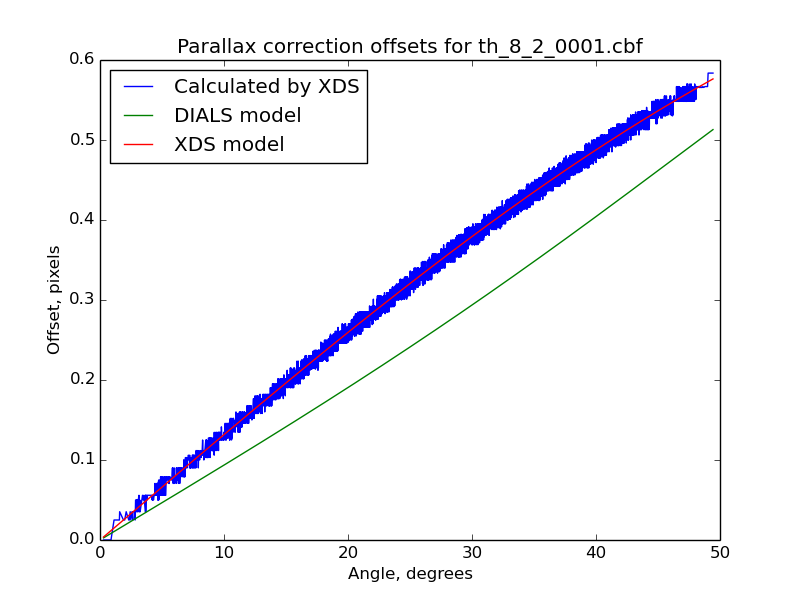
\includegraphics[scale=0.3]{corrections10000.png} \\ 
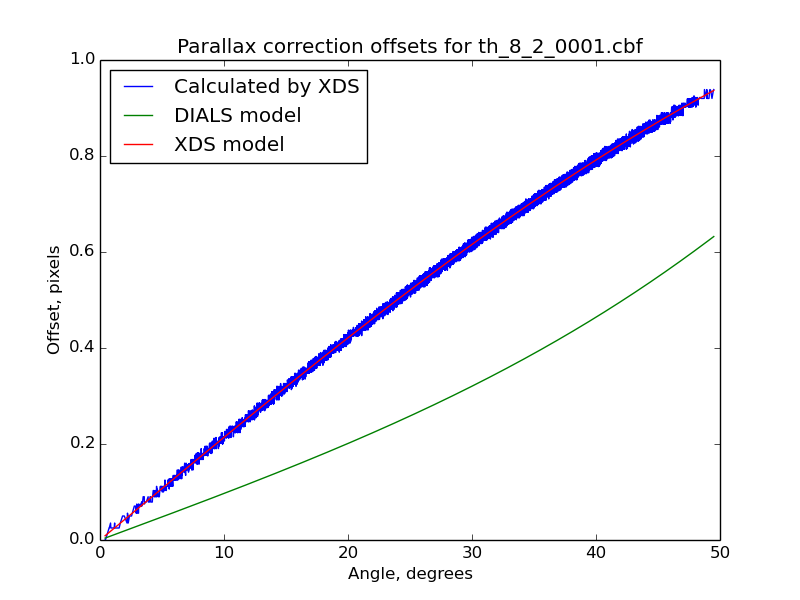
\includegraphics[scale=0.3]{corrections12000.png} &
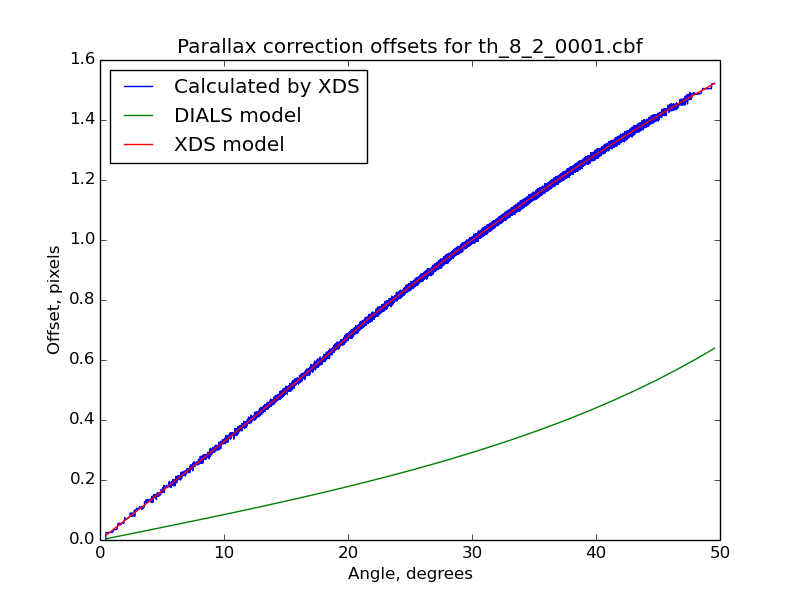
\includegraphics[scale=0.3]{corrections14000.png} \\
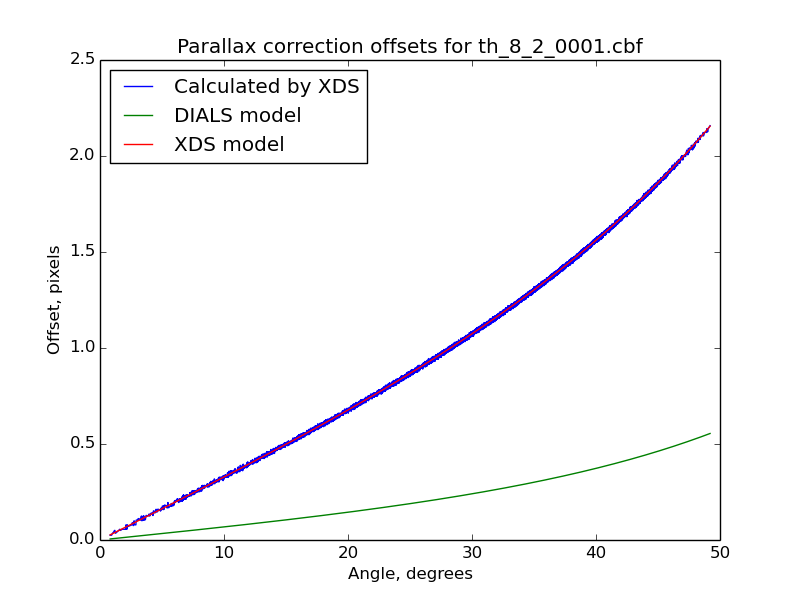
\includegraphics[scale=0.3]{corrections16000.png} & 
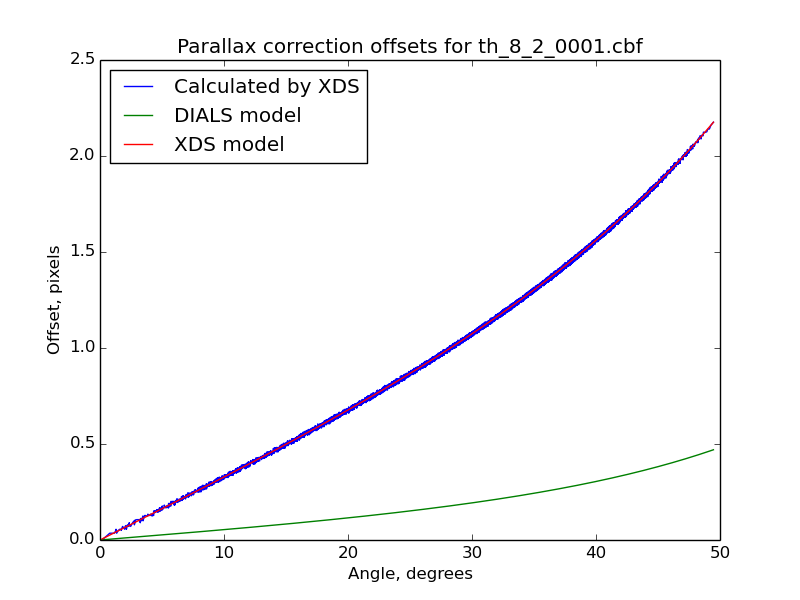
\includegraphics[scale=0.3]{corrections18000.png} \\
\end{tabular}
}

\section{Practical Implementation}

Though the overall offset has been derived here what is more useful is
the expected shift in $x$ and $y$ i.e. how the mapping deviates from a
perfect rectangular grid. This is easily derived from 

\begin{equation}
\theta_f = \cos^{-1} \underline{\hat{p}}.\underline{\hat{f}}
\end{equation}

\noindent
where $\theta_f$ is the angle between the incoming ray
$\underline{\hat{p}}$ and the fast direction $\underline{\hat{f}}$,
and similar for $\theta_s$ for the slow direction. Given the rules of
direction cosines it is easy to show that

\begin{equation}
<o_f> = \cos \theta_f \left( \frac{1}{\mu} - \left( \frac{t_0}{\cos
      \theta} + \frac{1}{\mu} \right) e^{- \frac{\mu t_0}{\cos \theta}} \right)
\end{equation}

\noindent 
and similar for $<o_s>$. The equation assumed for XDS may similarly be
decomposed to:

\begin{equation}
<o_f> = \rm{min}\left(\frac{\cos \theta_f}{\mu}, t_0 \frac{\cos
    \theta_f}{\cos \theta} \right)
\end{equation}

\noindent
where in both cases $\theta$ continues to be the angle between the ray
and detector normal. Turns out the errors in doing this are rather small:

{
\centering
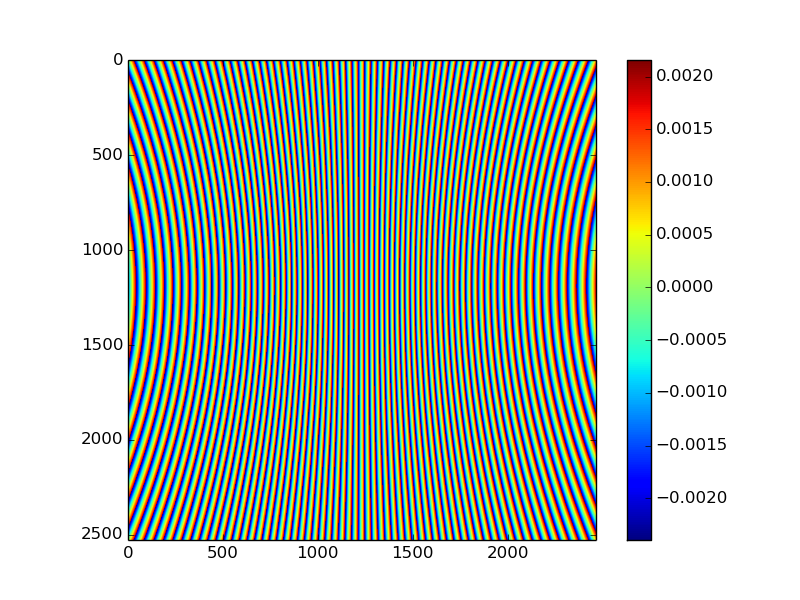
\includegraphics[scale=0.3]{dx.png}
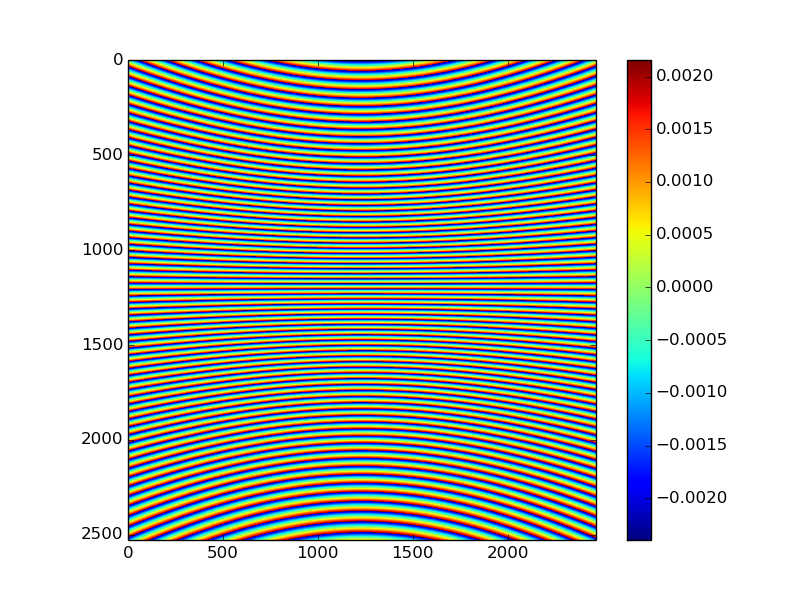
\includegraphics[scale=0.3]{dy.png}
}


\section{Next Steps}

Need to actually get experimental justification for these results
however am confident at this stage that they are (i) correct and (ii)
differ substantially from the model XDS uses. Now have a plan to get
some Monte Carlo simulations going, and also some offline test cases
where we ignore mm to pixel correction and apply manually.

\end{document}



